\subsection{Ловеринг операций и возможные стратегии}
\label{impl:lowering} % \index{Chapter8}

\newcommand{\divisible}{\mathop{\raisebox{-2pt}{\vdots}}}

Изучив особенности целевой архитектуры, перейдём к рассмотрению
конкретных стратегий ловеринга и их классификации. В связи с тем, что именно
работа с внешней память занимает большую часть времени, будем пытаться
оптимизировать еë. Как было упомянуто в одной из предыдущих глав, из-за малого
объëма внутренних кэшей данные приходится загружать частями, при этом каждая часть,
возможно, будет загружена несколько раз. В связи с этим, уменьшение количества
повторных загрузок --- самый простой способ оптимизации, а стратегия разбиения,
при которой достигается наименьшее количество повторных загрузок, будет считаться
нами наиболее оптимальной.

\subsubsection{Умножение матриц}

Умножение матриц в диалекте \texttt{ascend} представлено оператором \texttt{matmul}:

\begin{lstlisting}
func.func @kernel_func(
    %matrixA: memref<48x32x16x16xf16, 1>,
    %matrixB: memref<48x48x16x16xf16, 1>,
    %matrixC: memref<48x32x16x16xf16, 1>) {
    ascend.matmul(%matrixA, %matrixB, %matrixC) : memref<48x32x16x16xf16, 1>, memref<48x48x16x16xf16, 1>, memref<48x32x16x16xf16, 1>
    return
}
\end{lstlisting}

На вход оператор примает три многомерных массива, соответствующих матрицам
$A$, $B$, $C$ матричного умножения $C = A \times B$. Все три матрицы хранятся
в формате \texttt{Nz}, это сделано для удобства, т.~к. в реальных нейронных сетях
несколько умножений могут идти подряд, при этом результат предыдущего
передаётся на вход следующего. Привести кусок матрицы к необходимому формату
(\texttt{Zz} или \texttt{Zn}) не является проблемой при правильном использовании
операций копирования из GM в L1 и загрузки из L1 в L0. Число $1$ в конце каждого
\texttt{memref} означает, что массив находится в первом адресвом пространстве, что
соответствует памяти GM.

Теперь перейдём к тому, каким образом можно реализовать ловеринг и
оптимизировать количество копирований. Согласно статье FIXME, можно выделить
три основные стратегии: \textit{input stationary (IS)}, \textit{weight stationary (WS)}
и \textit{output stationary (OS)}. Отметим, что в данной статье рассматривается
операция свёртки, но всё перечисленное в ней верно и для умножения матриц.
Все три стратегии имеют общую идею: умножение производится блочно, блок одной из
матриц <<фиксируется>> ($A$ для IS, $B$ для WS и $C$ для OS), после чего
перебираются всевозможные блоки других матриц. Наглядное объяснение этого
процесса можно увидеть на картинке. После перебора выбирается другой блок и
операция повторяется.

\begin{figure}[h!]
    \centering
    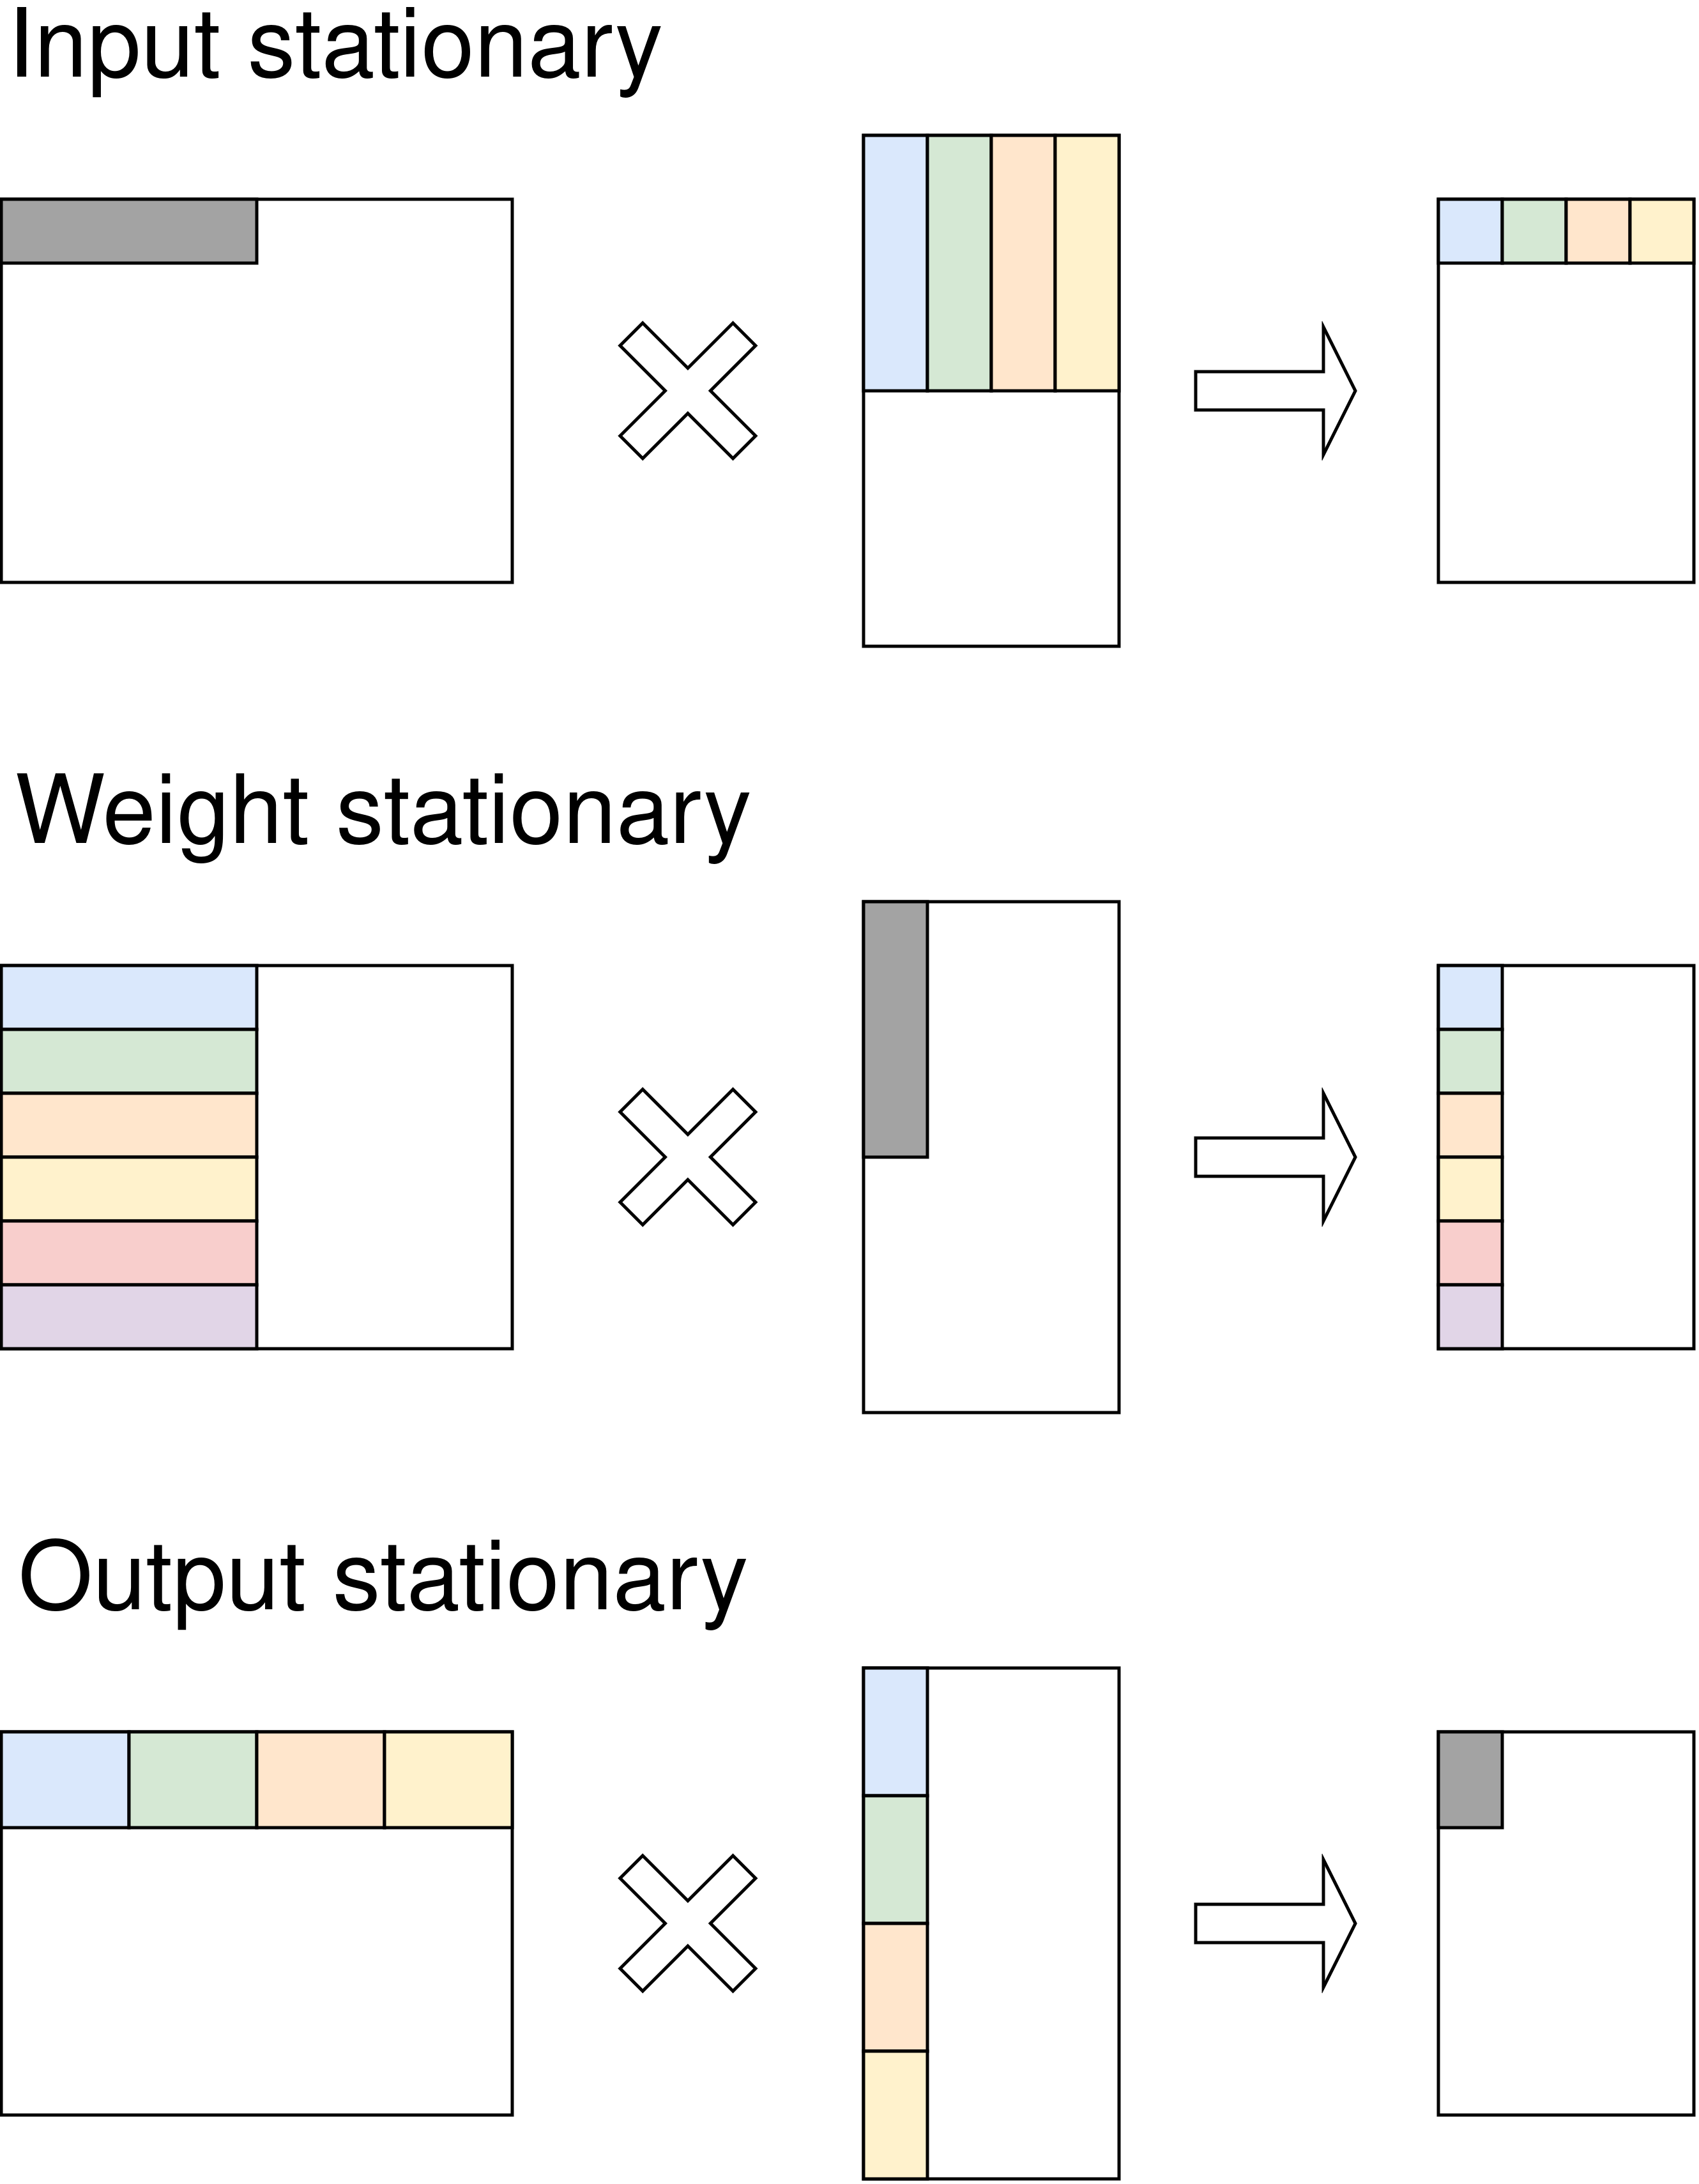
\includegraphics[scale=0.1]{Strategies.drawio.png}
    \caption{Стратегии для умножения матриц}
\end{figure}

Перечисленные стратегии описывают порядок обхода матриц по их блокам, но ничего
не говорят о размерах самих блоков. Пара стратегия + разбиение задаёт конкретное
исполнение, задача же состоит в том, чтобы выбрать исполнение, дающее
максимальную производительность. Для теоритического предсказания оптимального
исполнения нами была предложена метрика, соответствующая количеству загруженной
памяти. Опишем её более формально. Пусть матрица $A$ имеет размеры $M \times N$, а
матрица $B$ --- $N \times K$, тогда $C$ --- матрица $M \times K$. Таким образом,
матрицы описываются тройкой $(M, N, K)$. Аналогично, разбиение на блоки
описывается тройкой $(m, n, k)$. Будем рассматривать только такие конфигурации,
при которых блочное умножение можно выполнить за одну инструкцию, а выполнение
перебора блоков матриц при фиксации одного из них не требует выгрузки и загрузки
промежуточных результатов. В силу этих ограничений можно считать, что для IS
$k = K$ или $n = N$, а для WS --- $m = M$ или $n = N$.

Рассмотрим IS стратегию. Каждой загрузке матрицы $m \times n$ соответстует
$\frac{K}{k}$ загрузок матриц $n \times k$. Повторяется это действие
$\frac{MN}{mn}$ раз. Таким образом, общее количество загруженной памяти
составляет:

\[
    \Sigma_{IS} = \left( mn + nk ~ \frac{K}{k} \right) \frac{MN}{mn} = MN + \frac{MNK}{m}
\]

Аналогичным образом можно получить метрики для других стратегий:

\[
    \Sigma_{WS} = KN + \frac{MNK}{k}
\]

\[
    \Sigma_{OS} = MNK ~ \frac{m + k}{mk}
\]

На тройку $(m, n, k)$ должны быть наложены ограничения, связанные с размерами буферов.
Если считать, что элементы входных матриц имеют тип \texttt{float 16}, а выходной ---
\texttt{float 32} (это соответствует вычислениям на Ascend с повышенной точностью) тогда:

\[
\begin{cases}
    M, N, K, m, n, k \divisible 16 \\
    mn \leqslant 2^{15} \\
    nk \leqslant 2^{15} \\
    mk \leqslant 2^{16}
\end{cases}
\]

Итак, загружаемая память должна быть минимизирована, т.~е. $\Sigma \rightarrow \min$
Из эмпирических наблюдений (речь о которых пойдёт далее), при прочих равных используемая
память должна быть максимизирована:

\[
\begin{cases}
    mn \rightarrow \max \\
    nk \rightarrow \max \\
    mk \rightarrow \max
\end{cases}
\]

Для проверки гипотезы был разработан тестовый бенчмарк, замеряющий время
исполнения при различных конфигурацях. Гипотеза, изложенная выше, подтвердилась.
Если рассматривать типичные размеры умножаемых матриц в нейросетях (например,
BERT) --- $(512, 768, 768)$, то оказывается, что OS --- наиболее оптимальная
стратегия, а $(256, 128, 256)$ --- оптимальная конфигурация.

FIXME графики

OS стратегия была реализована в компиляторе на инфраструктуре MLIR в виде
понижения оператора \texttt{ascend.matmul} до цикла на диалектах cce,
affine и memref. Ниже приведён псевдокод алгоритма:

\begin{lstlisting}
func ascend.matmul(matrixA, matrixB, matrixC) {
    for (x = [0, M / m)) {
        for (y = [0, K / k)) {
            c = empty_buf(m, k)
            for (sum_part = [0, N / n)) {
                a = empty_buf(m, n)
                b = empty_buf(n, k)
                load_part(a, matrixA, sum_part, y)
                load_part(b, matrixB, x, sum_part)
                cce.mad(a, b, c)
            }
            store_part(matrixC, c, x, y)
        }
    }
}
\end{lstlisting}

Подчеркнём, что в реальности алгоритм имеет несколько особенностей, не
отражённых в псевдокоде. Во-первых, учитывается фрактализация матриц (их формат
хранения). Несмотря на то, что в L0A и L0B матрицы должны лежать в формате Zz и Zn
соответственно, в памяти GM они хранятся в формате Nz (это сделано для выполнения
нескольких умножений подряд без выполнения промежуточных фрактализаций). Изменение
формата происходит в ходе загрузки матриц во внутренни буферы. Во-вторых,
операции, названные в псевдокоде \texttt{load\_part} для $A$ и $B$ и \texttt{store\_part}
для $C$, состоят из двух этапов, для каждой матрицы по-разному:
$A: GM \rightarrow L1 \rightarrow L0A$, $B: GM \rightarrow L1 \rightarrow L0B$,
$C: L0C \rightarrow UB \rightarrow GM$. В-третьих, поддержана операция
\texttt{ascend.batch\_matmul}, которая производит умножение нескольких пар матриц.

\subsubsection{Фрактализация и дефрактализация}

Как было написано ранее, перемножение матриц требует особый формат хранения,
при этом было решено передавать на вход оператора умножения в формате Nz.
По этой причине необходимо матрицы, поступающие на вход нейронной сети, заранее
фрактализовать (т.е. поменять формат хранения). Обратное действие
(дефрактализация) необходимо для матрицы на выходе. Отметим, что далее речь
будет идти только о фрактализации, т.к. все преобразования линейны и
дефрактализация будет представлять собой действия фрактализации, выполненные в
обратном порядке. Рассмотрим фрактализацию на примере матрицы
$(512 \times 768)$. В формате Nz она будет иметь вид
$48 \times 32 \times 16 \times 16$. В скалярном коде фрактализация имеет
следующий вид:

\begin{lstlisting}
half src[512][768];
half dst[48][32][16][16];

for (i = [0, 48))
  for (j = [0, 32))
    for (k = [0, 16))
      for (l = [0, 16))
        dst[i][j][k][l] = src[j * 16 + k][i * 16 + l];
\end{lstlisting}

Исполнение скалярного кода является медленным, по этой причине будем
использовать инструкцию scatter\_vnchwconv. Было реализовано два алгоритма.

\textit{Наивный алгоритм} работает циклом с частями $16 \times 768$, первый
scatter собирает матрицы в блоки $16 \times 16$, а второй транспонирует
блоки. Для преобразования всей матрицы происходит перебор этих кусочков,
а копирование в GM происходит по блокам с шагом 32 блока.

\begin{lstlisting}
half src[16][768];
half tmp[48][16][16]
half dst[48][16][16];

scatter_vnchwconv(
    src = src, dst = tmp,
    src_ptrs = {{0, 0}, {1, 0}, {2, 0}, ...},
    dst_ptrs = {{0, 0, 0}, {0, 1, 0}, {0, 2, 0}, ...},
    src_stride = {0, 16},
    dst_stride = {1, 0, 0},
    repeat = 48
);

scatter_vnchwconv(
    src = tmp, dst = dst,
    src_ptrs = {{0, 0, 0}, {0, 1, 0}, {0, 2, 0}, ...},
    dst_ptrs = {{0, 0, 0}, {0, 1, 0}, {0, 2, 0}, ...},
    src_stride = {1, 0, 0},
    dst_stride = {1, 0, 0},
    repeat = 48
);
\end{lstlisting}

\textit{Улучшенный алгоритм} позволяет задействовать всю память UB:

\begin{lstlisting}
half src[80][768];
half tmp[5][48][16][16]
half dst[48][16][5][16];

half src_reshape[16][5][48][16] = reshape(src)

scatter_vnchwconv(
    src = src_reshape, dst = tmp,
    src_ptrs = {{0, 0, 0, 0}, {1, 0, 0, 0}, {2, 0, 0, 0}, ...},
    dst_ptrs = {{0, 0, 0, 0}, {0, 0, 1, 0}, {0, 0, 2, 0}, ...},
    src_stride = {0, 0, 1, 0},
    dst_stride = {0, 1, 0, 0},
    repeat = 240
);

for (i = [0, 5))
    scatter_vnchwconv(
        src = tmp, dst = src,
        src_ptrs = {{i, 0, 0, 0}, {i, 0, 1, 0}, {i, 0, 2, 0}, ...},
        dst_ptrs = {{0, 0, i, 0}, {0, 1, i, 0}, {0, 2, i, 0}, ...},
        src_stride = {0, 1, 0, 0},
        dst_stride = {1, 0, 0, 0},
        repeat = 48
    );

half dst_logical_shape[48][5][16][16] = reshape(dst)
\end{lstlisting}

С его помощью обрабатывается часть $80 \times 768$. После разбиения матрицы
на части остаётся <<хвост>> $32 \times 768$, который обрабатывается аналогично.
Загрузка результата в GM происходит по 5 блоков. Отметим, что операция reshape
является исключительно логической и не изменяет порядок хранения элементов.

\subsubsection{Поэлементные операции}

На момент написания текста были реализованы некоторые бинарные операции
(сложение, вычитание, умножение, деление, максимум, минимум), преобразование
типов и операция <<зажима>>: $clamp(x, y, z) = \min(z, \max(x, y))$. Все они
работают по общему приниципу: если массив данных многомерный, он преобразуется
к одномерному. Далее массив разбивается на максимально возможные порции,
при которых в UB помещаются входные и выходные данные. Данные загружаются из
GM порциями, обрабатываются соответствующими векторными операции и ответ
выгружается. Отметим, что в силу того, что количество элементов в порции
может быть некратным количеству элементов, обрабатываемых за итерацию инструкции
(128 в случае \texttt{float 16} и 64 в случае \texttt{float 32} или
\texttt{int 32}), конец порции необходимо обработать отдельно, предварительно
изменив маску.

Также может возникнуть проблема, связанная с обработкой последней порции и
гранулярностью UB. Напомним, что в UB возможна заргузка данных, размер которых
кратен 32 байтам. Это означает, что если размер всего массива данных не кратен
32, то с загрузкой последней порции могут возникнуть случае. Решением этой
проблемы является загрузка <<с наложением>>: загрузка некоторую часть предыдущей
порции с целью выровнять размер. При этом это <<наложение>> обрабатывается и
выгружается повторно. Отметим, что такая схема не влияет на общую
производительность, т.~к. размер <<наложения>> пренебрежимо мал по сравнению
с размерами всего массива.

\subsection{Транспонирование}

Операция транспонирования в моделях нейронных сетей работает с многомерными
тензорами, по этой причине данную операцию корректнее называть <<перестановкой
измерений>>. В каком-то смысле эта операция является изменением формата хранения
данных, но более общим случаем. На данный момент поддержаны операции из BERT,
их можно представить в двух формах:

\textit{Первая форма} выражается формулой $dst_{ijk} = src_{ikj}$, т.~е.
является транспонированием нескольких матриц. Решается задача аналогично
поэлементным операциям за тем лишь исключением, что в данном случае используется
инструкция \texttt{scatter\_vnchwconv}, которая работает с матрицами
$16 \times 16$, что является гранулярностью в данном случае. Проблема, связанные
с гранулярностью, решается аналогично: алгоритм использует схему <<с наложением>>.

\textit{Вторая форма} выражается формулой $dst_{ijkl} = src_{ikjl}$. В данном
случае алгоритм осуществляет поблочное копирование из преположения, что размер
младшего измерения кратен 32 байтам.
